%!TEX root = practicum3.tex
\subsection*{Method}
	% Computing the path
	To compute the path from \t{p0} to \t{p1} over the three-dimensional surface defined by the triangulation $dtl$ we have adapted the method used for the second part of \autoref{s:c}. We have taken the following steps:
	\begin{enumerate}
		\item \label{alg:d:1} \t{t0} $:=$ the triangle containing \t{p0}.
		\item \label{alg:d:2} \t{t1} $:=$ the triangle containing \t{p1}.
		\item \label{alg:d:3} \t{p} $:=$ the projection of the point \t{p0} on triangle \t{t0}.
		\item \label{alg:d:4} \t{while t != t1}
			\begin{enumerate}
				\item \label{alg:d:while1} \t{e0} $:=$ \t{p}
				\item \label{alg:d:while2} \t{p} $:=$ the intersection of the line segment between \t{p0} and \t{p1} and the edge of the neighbouring triangle \t{n} of \t{t}, where \t{n} does not already contain a part of the path.
				\item \label{alg:d:while3} \t{t} $:=$ \t{n}
				\item \label{alg:d:while4} add the edge from \t{e0} to \t{p} to the list of edges.
			\end{enumerate}
		\item \label{alg:d:5} \t{e1} $:=$ the projection of the point \t{p1} on triangle \t{t1}.
		\item \label{alg:d:6} add the edge from \t{p} to \t{e1} to the list of edges.
	\end{enumerate}

	The method \t{find_neighbouring_edge_intersected_by_s}, see \autoref{lst:d:find_neighbouring_edge_intersected_by_s}, implements step \autoref{alg:d:while2} through \autoref{alg:d:while3}. This method is essentially the same as \t{find_intersected_edges}, see \autoref{lst:c:find_intersected_edges}, used in \autoref{s:c}. With the added computation of the projection, which is computed by \t{project_point_on_plane} defined in \autoref{lst:b:pointPlaneProjection}.

	All other mentioned steps are executed by the method \t{find_path}, see \autoref{lst:d:find_path}. After executing this method the global parameter \t{path_edges} contains all the edges on the path and \t{path_triangles} contains all triangles that are traversed when following the path. This list used in \t{find_neighbouring_edge_intersected_by_s} to ensure that we choose edge to intersect in such a way that we move towards \t{p1} along $s$. 

	Both \t{find_neighbouring_edge_intersected_by_s} and \t{find_path} use the method \t{get_triangle}. This method returns a triangle from the triangulation given an index in \t{triPts}, \t{neighs} or \t{cens} as a list of three-dimensional points, see \autoref{lst:d:get_triangle}.\\

	\lstinputlisting[float, firstline=253, lastline=265, label={lst:d:find_neighbouring_edge_intersected_by_s}, caption={The method \t{find_neighbouring_edge_intersected_by_s()}.}]{../assignment3D.py}

	\lstinputlisting[float, firstline=278, lastline=303, label={lst:d:find_path}, caption={The method \t{find_path()}.}]{../assignment3D.py}

	\lstinputlisting[float, firstline=268, lastline=275, label={lst:d:get_triangle}, caption={The method \t{get_triangle()}.}]{../assignment3D.py}

	% Visualizing the path
	The path is visualised by adding drawing the line segments stored in \t{path_edges}, see \autoref{lst:d:display}. Two computed paths are visualized in \autoref{fig:d:results}.\\

	\lstinputlisting[float, firstline=134, lastline=142, label={lst:d:display}, caption={Part of the method \t{generate_dl()}.}]{../assignment3D.py}

	% Computing the length of the path
	The length of the path can be computed by adding the length of the line segments that from the path. To compute the length of one line segment we use the method \t{euclidean_distance} presented in \autoref{lst:d:euclidean_distance}. Adding these lengths gives the length of the path, see \autoref{lst:d:path_length}. The length of the path over $dtl_1$, the triangulation with vertices delivered by \t{generate_points}, is \num{548.360146342}. The length of the path over $dtl_2$, the triangulation with vertices delivered by \t{read_points}, is \num{577.574599559}.\\

	\lstinputlisting[float, firstline=306, lastline=308, label={lst:d:euclidean_distance}, caption={The method \t{euclidean_distance()}.}]{../assignment3D.py}

	\lstinputlisting[float, firstline=311, lastline=313, label={lst:d:path_length}, caption={The method \t{path_length()}.}]{../assignment3D.py}

	The line segments defining the path from \t{p0} to \t{p1} are printed when the program is executed. The paths are visualized in \autoref{fig:d:results}.

	\begin{figure}
		\centering
		\begin{subfigure}[b]{0.45\textwidth}
			\centering
			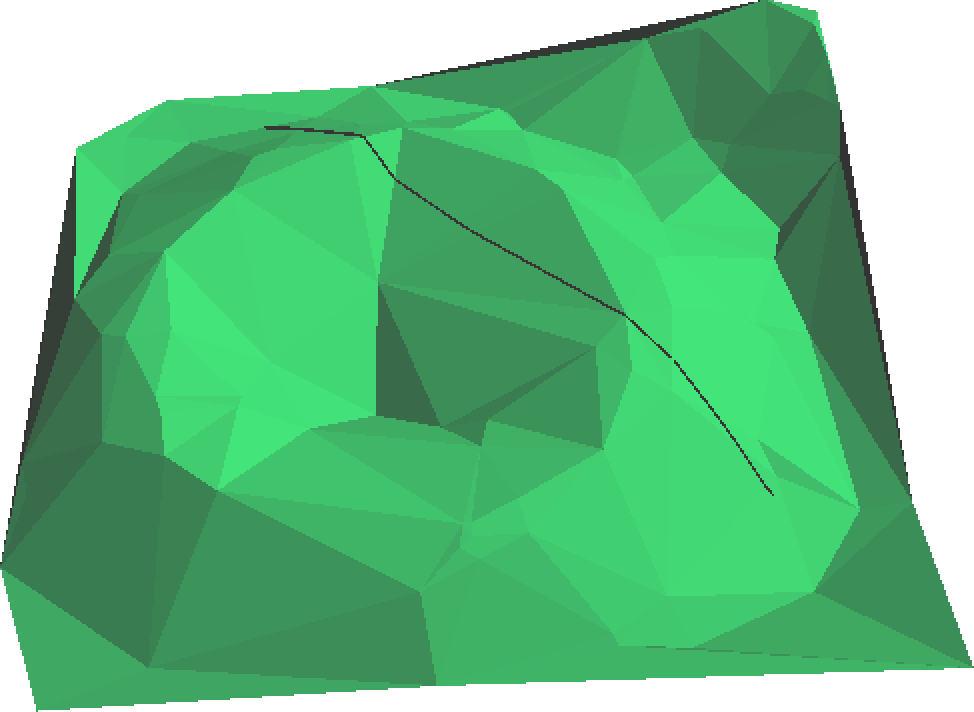
\includegraphics[width=0.9\textwidth]{./img/d_result1}
			\caption{$dlt_1$ (\t{generate_points()})}
			\label{subfig:d:result1}
		\end{subfigure}
		\begin{subfigure}[b]{0.45\textwidth}
			\centering
			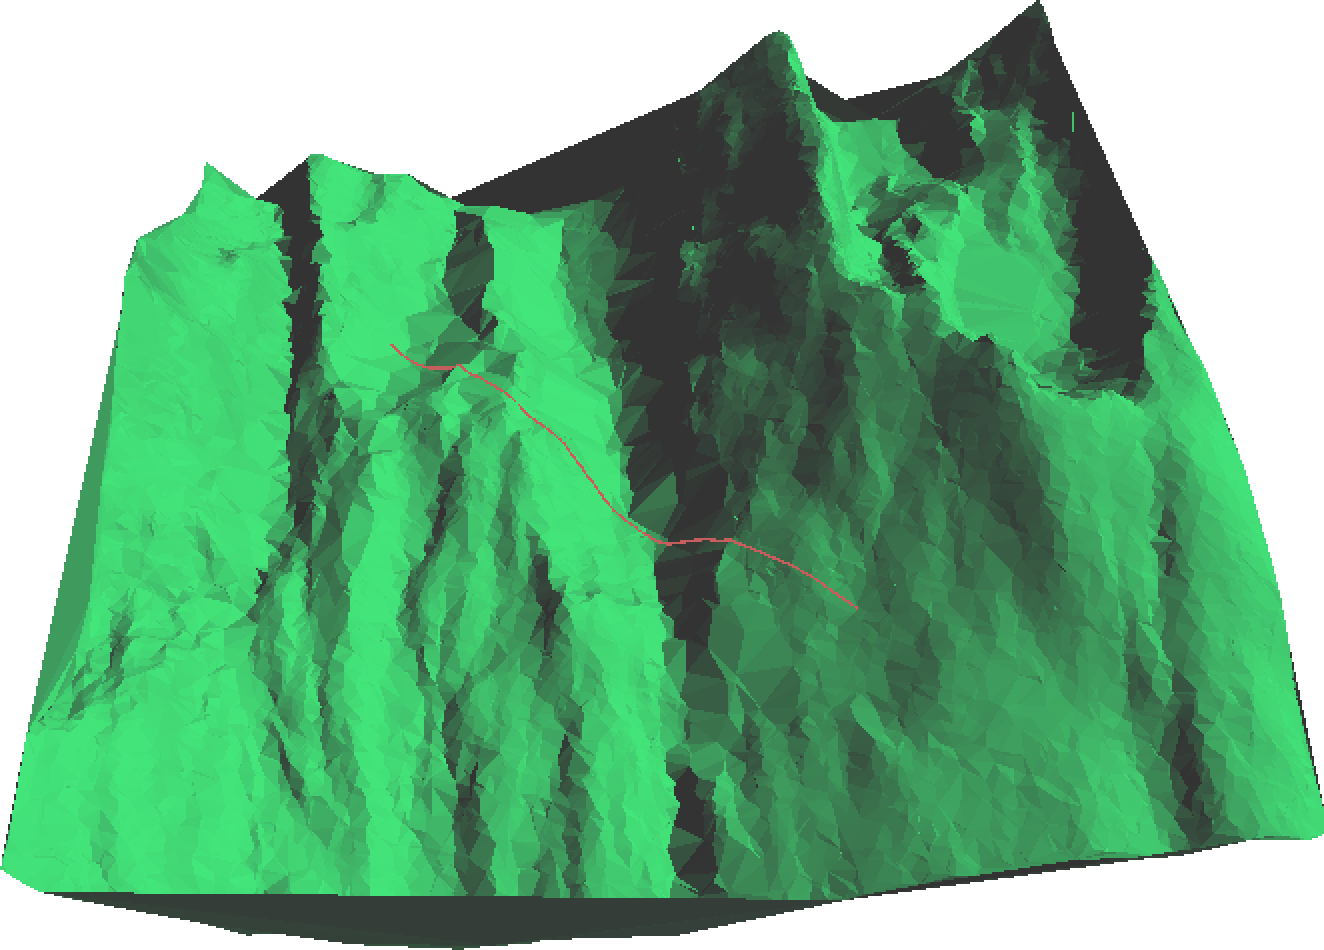
\includegraphics[width=0.9\textwidth]{./img/d_result2}
			\caption{$dlt_2$ (\t{read_points()})}
			\label{subfig:d:result2}
		\end{subfigure}	
		\caption{A path from \t{p0} to \t{p1}, the points on which the triangulation are based are delivered by (\subref{subfig:d:result1}) \t{generate_points} or (\subref{subfig:d:result2}) \t{read_points}.}
		\label{fig:d:results}
	\end{figure}

	\todo[inline]{Explain why the Delaunay triangulation is very well suited for this problem.
Can you think of a way of verifying the correctness of your path-length calculation for simplified input data?}